\documentclass[12pt]{article}
\usepackage[utf8]{inputenc}
\usepackage{graphics}
\usepackage{graphicx}
\usepackage{float}
\usepackage{hyperref}
\hypersetup{
	colorlinks=true,
	linkcolor=blue,
	filecolor=magenta,      
	urlcolor=cyan,
}

\title{Release plan}
\author{Thomas van Dongen, Koen Schilders}
\date{7 februari 2018}

\begin{document}


% De titelpagina
\begin{titlepage}
\maketitle
\end{titlepage}



% Hier worden alle branches beschreven
\section{Omschrijving per branch}
\begin{figure}[H]
	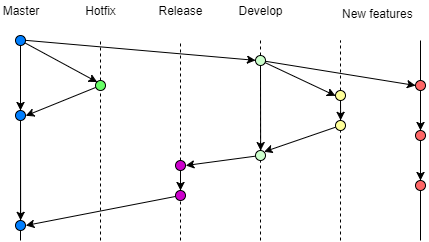
\includegraphics[width=\textwidth]{images/SOP6_Release.png}
	\caption{Het releaseplan.}
\end{figure}
\subsection{Master}
De master is de branch waar een geteste releases staan, bedoelt voor deployment. Het is mogelijk om een ontwikkelstraat op te zetten die een nieuwe commit naar de master automatisch build en deployed naar bijvoorbeeld de Appstore.
\subsection{Hotfix}
Als er een ernstige bug gevonden is in de master branch is het nodig om deze direct op te lossen. Een hotfix dient dan in de hotfix branch gemaakt te worden. Hiervoor wordt de build van de master gepulled, en een hotfix gemaakt. Vervolgens wordt deze naar de master gepushed als nieuwe versie.
\subsection{Release}
De build van develop wordt naar de release branch gepushed als deze compleet is. Het QA-team kan deze versie testen. Bugs kunnen in deze branch gefixed worden, waarna het QA-team deze versie opnieuw test. Als de versie de groene vlag krijgt, en er geen bugs gevonden zijn, kan de master branch deze versie pullen.
\subsection{Develop}
De develop branch wordt gebruikt als start punt voor het ontwikkelen van nieuwe features. Er wordt vanaf deze branch een nieuwe branch gemaakt en daar wordt verder op gewerkt. Er wordt dus nooit ontwikkeld op deze branch.
\subsection{New features}
Om er voor te zorgen dat het ontwikkelen van nieuwe branches goed verloopt maken we gebruik van feature branches. Elke nieuwe feature krijgt zijn eigen branch. Pas wanneer de feature af is wordt deze weer gemerged met de develop branch. De feature branch wordt na de merge verwijdert.



% Hier wordt het releaseplan gemaakt in Git beschreven
\pagebreak
\section{Releaseplan in Git}
\begin{figure}[H]
	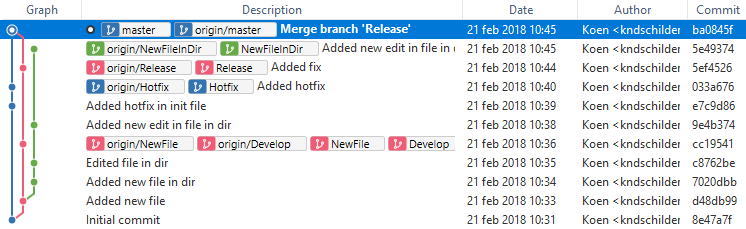
\includegraphics[width=\textwidth]{images/ReleasePlanInGit.png}
	\caption{Het releaseplan weergegeven in Sourcetree.}
\end{figure}
Het releaseplan beschreven in sectie 1 staat hierboven uitgewerkt in Sourcetree. In Sourcetree is het eenvoudig om een nieuwe branch aan te maken:

\begin{figure}[H]
	\centering
	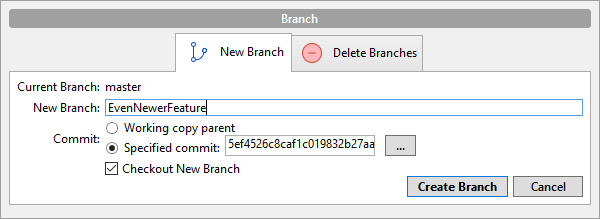
\includegraphics[width=\textwidth]{images/NewBranch.png}
\end{figure}

Er kan gekozen worden om de branch te beginnen vanaf een specifieke commit. Hiermee hebben we de opzet van het releaseplan nagemaakt.
\href{https://github.com/kndschilders/ReleasePlanGitTest}{Hier}
staat de volledige git repository. De branch 'NewFile' bestaat nog ter illustratie, maar zou in een echte production verwijderd moeten worden.

% Nadere toelichting van Canvas vragen
\pagebreak
\section{Kwaliteit}
De kwaliteit van een applicatie voorspelt onder andere hoe goed de applicatie onderhouden kan worden. De kwaliteit van een applicatie omvat veel zaken, zoals de codekwaliteit, testen en documentatie.

\subsection{Codekwaliteit}
% Wanneer is code goed genoeg om mee te mogen in een release?
Een applicatie met code van slechte kwaliteit maakt het onderhouden van de applicatie op lange termijn erg lastig, vooral als er nieuwe ontwikkelaars aan gaan werken. Daarnaast is de kans op bugs waarschijnlijker bij code van slechte kwaliteit.
\newline
Codekwaliteit is een rekbaar begrip. Daarom hanteren we de volgende eisen waaraan code van goede kwaliteit aan moet voldoen:

\begin{description}
	\item[Eis 1] Lorem ipsum dolor sit amet
	\item[Eis 2] Lorem ipsum dolor sit amet
	\item[Eis 3] Lorem ipsum dolor sit amet
\end{description}

\subsection{Testing}
% Hoe en waar gaat de nieuwe feature getest worden?
Testen worden gebruikt om de functionaliteit van een applicatie te controleren. Tijdens het ontwikkelen moet een individuele feature natuurlijk getest worden alvorens het naar de development-branch wordt gepushed. Dit testen gebeurt in de feature-branch van de feature. Omdat er gewerkt wordt volgens het Test-Driven Development principe is het eenvoudig de feature te testen door de JUnit-tests uit te voeren. Als deze JUnit-tests geslaagd zijn is de feature 'af', en kan deze naar de development-branch.
\newline
Het is aan te raden om voor de belangrijkste klassen en methodes een code coverage van 100\% te hebben. Code coverage voor getters en setters zijn onnodig en tijdrovend. Daarom is 100\% code coverage voor de gehele applicatie geen goede tijdsinvestering.

\subsection{Documentatie}
% Wat zijn de eisen aan dingen als documentatie etc. voordat de feature klaar is (definition of done)?
Documentatie is noodzakelijk voor het onderhouden van de applicatie, voornamelijk als de applicatie voor langere tijd moet worden onderhouden. Documentatie kan minimaal of zeer uitgebreid zijn. De code van elke feature moet minstens voldoen aan de 1\textsuperscript{ste} van de volgende eisen:

\begin{enumerate}
	\item Code documentatie (Javadoc) van belangrijkste klassen en methodes.
	\item Comments binnen de belangrijkste methodes.
	\item Code documentatie (Javadoc) van alle klassen en methodes binnen de applicatie.
	\item Comments binnen de gehele applicatie.
\end{enumerate}
% TODO uitbreiden

\noindent Naast code documentatie is het verstandig een handleiding te maken voor het gebruik van de applicatie. In deze handleiding wordt beschreven hoe de applicatie ... %TODO uitbreiden

\pagebreak
\section{Eisen voor release}
% Wat zit er allemaal in een release?

\subsection{Versienummers}
% Wat doe je met versienummers?

\end{document}